\documentclass{article}
\usepackage{amsmath}
\usepackage{titlesec}
\usepackage{graphicx}
\usepackage[margin=1in]{geometry}

% Title, date, and author
\title{Exercise 1}
\author{Your Name, Collaborator's Name}
\date{\today}

\titleformat{\section}
  {\normalfont\normalsize\bfseries} % Format: font style, size, and weight
  {\thesection}{1em} % Label format and spacing
  {}
  \renewcommand{\thesubsection}{\thesection.\alph{subsection}}

\titleformat{\subsection}
  {\normalfont\small\bfseries} % Format: font style, size, and weight
  {\thesubsection}{1em} % Label format and spacing
  {}
\titleformat{\subsubsection}
  {\normalfont\small\bfseries} % Format: font style, size, and weight
  {\thesubsubsection}{1em} % Label format and spacing
  {}

\begin{document}
\begin{titlepage}
    \centering
    \vspace*{1in}
    
    {\Huge\bfseries Exercise 1\par}
    \vspace{1.5cm}
    {\Large \today\par}
    \vspace{1.5cm}
    {\Large\itshape Antonio Pampalone\\ Giuseppe Pisante\\ Martina Raffaelli\par}
    
    \vfill
    
\includegraphics[width=0.3\textwidth]{FAU-Logo.png}\par\vspace{1cm} % Adjust the width as needed
   
\end{titlepage}

\newpage
\small

\section{Elementary Vector Calculus}
 
\subsection{Gradient of a scalar $\phi$:}
    \begin{equation}
        grad(\phi) = \nabla \phi = \frac{\partial \phi}{\partial x_i} = \left( \frac{\partial \phi}{\partial x}, \frac{\partial \phi}{\partial y}, \frac{\partial \phi}{\partial z} \right)
    \end{equation}
\subsection{Divergence of the velocity vector $\vec{u}$:}
    \begin{equation}
        div(\vec{u}) = \nabla \cdot \vec{u} = \frac{\partial u_i}{\partial x_i} = \frac{\partial u}{\partial x} + \frac{\partial v}{\partial y} + \frac{\partial w}{\partial z}
    \end{equation}
\subsection{Curl of the velocity vector (vorticity):}
    \begin{equation}
        rot(\vec{u}) = \nabla \times \vec{u} = 
        \begin{vmatrix}
        \hat{i} & \hat{j} & \hat{k} \\
        \frac{\partial}{\partial x} & \frac{\partial}{\partial y} & \frac{\partial}{\partial z} \\
        u & v & w
        \end{vmatrix}
    = \left( \frac{\partial w}{\partial y} - \frac{\partial v}{\partial z}, \frac{\partial u}{\partial z} - \frac{\partial w}{\partial x}, \frac{\partial v}{\partial x} - \frac{\partial u}{\partial y} \right)
    \end{equation}
\subsection{Material derivative of a scalar:}
    \begin{equation}
        \frac{D\phi}{Dt} = \frac{\partial \phi}{\partial t} + (\vec{u} \cdot \nabla) \phi = \frac{\partial \phi}{\partial t} + u \frac{\partial \phi}{\partial x} + v \frac{\partial \phi}{\partial y} + w \frac{\partial \phi}{\partial z}
    \end{equation}
\subsection{Material derivative of the velocity vector:}
    \begin{equation}
        \begin{aligned}
        \frac{D\vec{u}}{Dt} &= \frac{\partial \vec{u}}{\partial t} + (\vec{u} \cdot \nabla) \vec{u} \\
        &= \left(\frac{\partial u}{\partial t}, \frac{\partial v}{\partial t}, \frac{\partial w}{\partial t}\right) + \left(\frac{\partial u}{\partial x} + \frac{\partial v}{\partial y} + \frac{\partial w}{\partial z}\right) \left(u, v, z\right) \\
        &= \left(\frac{\partial u}{\partial t}, \frac{\partial v}{\partial t}, \frac{\partial w}{\partial t}\right) + \frac{\partial u_i}{\partial x_i} \left(u, v, z\right)
        \end{aligned}
    \end{equation}
\subsection{Rate-of-strain-tensor:}
    \begin{equation}
        S = \frac{1}{2} \left(\nabla \vec{u} + (\nabla \vec{u})^T\right) = \frac{1}{2} \begin{pmatrix} 
            2 \frac{\partial u}{\partial x} & \frac{\partial u}{\partial y} + \frac{\partial v}{\partial x} & \frac{\partial u}{\partial z} + \frac{\partial w}{\partial x} \\
            \frac{\partial v}{\partial x} + \frac{\partial u}{\partial y} & 2 \frac{\partial v}{\partial y} & \frac{\partial v}{\partial z} + \frac{\partial w}{\partial y} \\
            \frac{\partial w}{\partial x} + \frac{\partial u}{\partial z} & \frac{\partial w}{\partial y} + \frac{\partial v}{\partial z} & 2 \frac{\partial w}{\partial z}
            \end{pmatrix}
    \end{equation}
\subsection{Divergence of the rate-of-strain tensor:}
    \begin{equation}
        \begin{aligned}
        \nabla \cdot \mathbf{S} &= \frac{\partial S}{\partial x_i} = \frac{1}{2} \left(\frac{\partial}{\partial x}, \frac{\partial}{\partial y}, \frac{\partial}{\partial z}\right) \begin{pmatrix} 
        2 \frac{\partial u}{\partial x} & \frac{\partial u}{\partial y} + \frac{\partial v}{\partial x} & \frac{\partial u}{\partial z} + \frac{\partial w}{\partial x} \\
        \frac{\partial v}{\partial x} + \frac{\partial u}{\partial y} & 2 \frac{\partial v}{\partial y} & \frac{\partial v}{\partial z} + \frac{\partial w}{\partial y} \\
        \frac{\partial w}{\partial x} + \frac{\partial u}{\partial z} & \frac{\partial w}{\partial y} + \frac{\partial v}{\partial z} & 2 \frac{\partial w}{\partial z}
        \end{pmatrix} \\
        &= \frac{1}{2}\left(2\frac{\partial^2 u}{\partial x^2} + \frac{\partial^2 v}{\partial x \partial y} + \frac{\partial^2 u}{\partial y^2} + \frac{\partial^2 w}{\partial x \partial z} + \frac{\partial^2 u}{\partial z^2}, \right. \\
        &\quad \left. \frac{\partial^2 u}{\partial y^2} + \frac{\partial^2 v}{\partial x \partial y} + 2 \frac{\partial^2 v}{\partial y^2} + \frac{\partial^2 w}{\partial y^2} + \frac{\partial^2 v}{\partial y \partial z}, \right. \\
        &\quad \left. \frac{\partial^2 u}{\partial x \partial z} + \frac{\partial^2 w}{\partial x^2} + \frac{\partial^2 v}{\partial x \partial z} + \frac{\partial^2 w}{\partial y^2} + 2 \frac{\partial^2 w}{\partial z^2}\right)
        \end{aligned}
        \end{equation}


\section{Global versus local rotation}

\subsection{Sketch of the flows:}
\subsubsection{Line vortex flow: \textnormal{$\vec{u} = [u_r, u_\theta, u_z] = \left[0, -\frac{\alpha}{r}, 0\right]$ }}
\begin{figure}[h!]
    \centering
    \begin{tabular}{cc}
        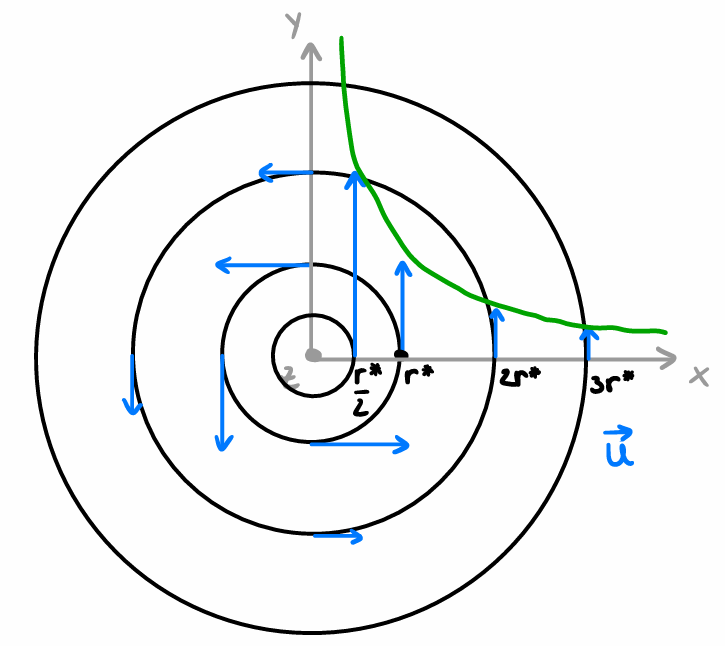
\includegraphics[width=0.20\textwidth]{imm_1.1.png} &
        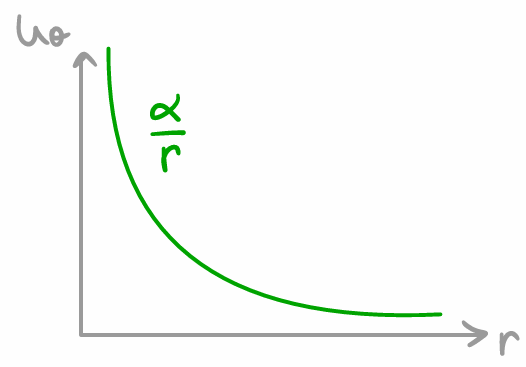
\includegraphics[width=0.20\textwidth]{imm_1.2.png}
    \end{tabular}
    \caption{Line vortex flow}
    \label{fig:mie_immagini}
\end{figure}
\subsubsection{Plane shear flow: \textnormal{$\vec{u} = [u, v, w] = \left[\beta y, -0, 0\right]$}} 
\begin{figure}[h!]
    \centering
    \begin{tabular}{cc}
        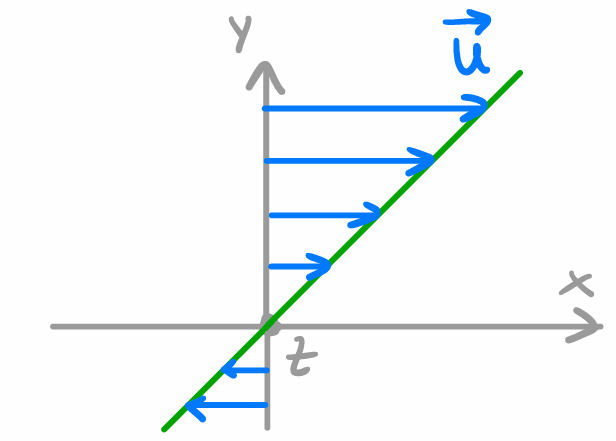
\includegraphics[width=0.20\textwidth]{imm_2.1.png} &
        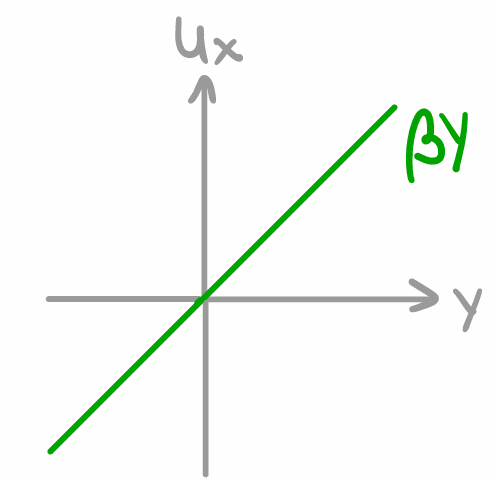
\includegraphics[width=0.20\textwidth]{imm_2.2.png}
    \end{tabular}
    \caption{Plane shear flow}
    \label{fig:mie_immagini}
\end{figure}
\subsubsection{Flow between rotating cylinders: \textnormal{$\vec{u} = [u_r, u_\theta, u_z] = \left[0, Ar + \frac{B}{r}, 0\right]$}} 
\begin{figure}[h!]
    \centering
    \begin{tabular}{cc}
        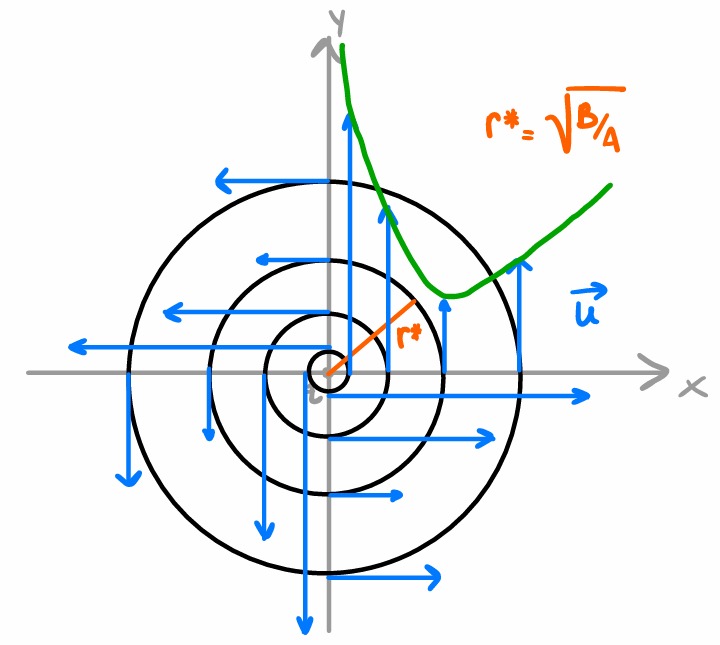
\includegraphics[width=0.20\textwidth]{imm_3.1.png} &
        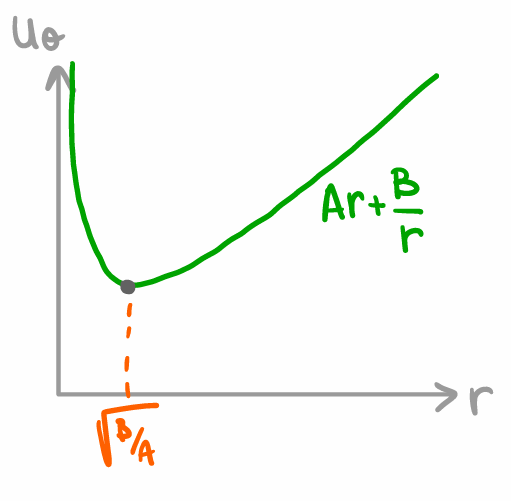
\includegraphics[width=0.20\textwidth]{imm_3.2.png}
    \end{tabular}
    \caption{Flow between rotating cylinders}
    \label{fig:mie_immagini}
\end{figure}


\subsection{Local and global rotations:}
To verify wheter a flow features a local/global rotation we need to compute its vorticity, which is a vector quantity defined as $\vec{\omega} = \nabla \times \mathbf{u}$.
\subsubsection{Line vortex flow:}
For this specific flow we have that the vorticity vector is $\vec{\omega} = [0, 0, 0]$, so this flow does not show a local nor a global rotation since the vorticity is the null vector.
\subsubsection{Plane shear flow:}
Making usage of the previously delined formula for the vorticity, we find that $\vec{\omega}  = \left[0, 0, -\beta\right]$ which indicates that we have a shear-induced rotation around the $z$-axis. Also this flow does not feature a global rotation because it is characterized by a velocity gradient in the $y$-direction (shear) rather than a circular motion and this causes fluid elements to rotate locally due to the velocity differences at different $y$-positions, but there is no coordinated or structured rotation of the entire flow field. The flow is linear, not circular, so it doesn't exhibit global rotation. 
\subsubsection{Flow between rotating cylinders:}
As in the former cases we compute the vorticity: $\vec{\omega} = [0, 0, 2A]$. Also the third flow exibits a local rotation due to the non-zero vorticiy, but unlike the previous cases the rotating cylinders create a structured and circular flow with a consistent rotational effect through the domain. 

In all three cases, we could have reached similar conclusions by observing the graphs shown above.


\section{Mass Conservation}

The continuity equation (mass conservation) states that the change of mass per unit time in an infinitesimal control volume (CV) is equal to the difference between the mass inflow and outflow rate of the CV. Assume an infinitesimally small fluid element fixed in space (Eulerian) with velocity vector $\mathbf{u}$ and density $\rho$ the net outflow in x-direction is given by:

\begin{equation}
\rho u_1 + \frac{\partial \rho u_1}{\partial x} dx \, dy \, dz - \rho u_1 dy \, dz = \frac{\partial \rho u_1}{\partial x} dx \, dy \, dz
\end{equation}

Similarly the net outflow in y-direction and the net outflow in z-direction are given by:

\[
\frac{\partial \rho u_2}{\partial y} dx \, dy \, dz \quad \frac{\partial \rho u_3}{\partial z} dx \, dy \, dz
\]

Therefore the net mass flow out of the element is given by:

\[
\frac{\partial \rho u_1}{\partial x} dx \, dy \, dz + \frac{\partial \rho u_2}{\partial y} dx \, dy \, dz + \frac{\partial \rho u_3}{\partial z} dx \, dy \, dz
\]

The rate of change of mass within the control volume is given by:

\[
\frac{\partial \rho}{\partial t} dx \, dy \, dz
\]

Combining the previous equations we can obtain the continuity equation:

\[
\frac{\partial \rho u_1}{\partial x} dx \, dy \, dz + \frac{\partial \rho u_2}{\partial y} dx \, dy \, dz + \frac{\partial \rho u_3}{\partial z} dx \, dy \, dz = - \frac{\partial \rho}{\partial t} dx \, dy \, dz
\]

Leading to the final notation:

\[
\frac{\partial \rho}{\partial t} + \frac{\partial \rho u_i}{\partial x_i} = \frac{\partial \rho}{\partial t} + \nabla \cdot (\rho \mathbf{u}) = 0
\]

For an incompressible flow (constant density $\rho$) the continuity equation simplifies to:

\[
\frac{\partial u_i}{\partial x_i} = \nabla \cdot \mathbf{u} = 0
\]

Written for a Cartesian coordinate system $(x, y, z)$ becomes:

\[
\frac{\partial u}{\partial x} + \frac{\partial v}{\partial y} + \frac{\partial w}{\partial z} = 0
\]

This means that the divergence of the velocity field is zero indicating that fluid volume is conserved.

\section{Non-dimensional Navier–Stokes Equations}

The Navier–Stokes equations of an incompressible isothermal Newtonian fluid are:

\[
\frac{\partial u_i}{\partial x_i} = 0
\]

\[
\rho \frac{\partial u_i}{\partial t} + u_j \frac{\partial u_i}{\partial x_j} = - \frac{\partial p}{\partial x_i} + \frac{\partial \tau_{ij}}{\partial x_j}
\]

The mass conservation means the fluid density remains constant and there is no volume change at any point in the fluid. The conservation of momentum means that changing the momentum is equivalent to a force. In particular, the first term is the local acceleration which represents the rate of change of velocity with time, while the second term is the convective acceleration, which represents the rate of change of velocity due to spatial variations in the velocity field. On the right-hand side, there are the pressure gradient force that shows how the fluid accelerates due to pressure differences and the term representing the viscous forces in the fluid which resist deformation due to viscosity.

For a Newtonian fluid, the shear-stress tensor $\tau_{ij}$ is given by:

\[
\tau_{ij} = 2 \mu S_{ij}
\]

where $S_{ij}$ is the rate of strain tensor defined as:

\[
S_{ij} = \frac{1}{2} \left( \frac{\partial u_i}{\partial x_j} + \frac{\partial u_j}{\partial x_i} \right)
\]

Substituting $\tau_{ij}$ in the momentum equation for an incompressible fluid this reduces to:

\[
\frac{\partial \tau_{ij}}{\partial x_j} = \mu \frac{\partial}{\partial x_j} \left( \frac{\partial u_i}{\partial x_j} + \frac{\partial u_j}{\partial x_i} \right) = \mu \frac{\partial^2 u_i}{\partial x_j \partial x_j}
\]

To obtain the dimensionless form, we introduce appropriate reference quantities and corresponding non-dimensional quantities (with *). In the example of pipe flow, it is natural to scale lengths with the pipe diameter $D$, velocities with the mean speed $U$, time with the ratio of length to mean velocity, while the natural scale for pressure is given by the product of density and the mean speed squared.

\[
x_i = D x_i^*, \quad u_i = U u_i^*, \quad t_i = \frac{L}{U} t_i^*, \quad p_i = \rho U^2 p_i^*
\]

Substitute these into the Navier-Stokes equations, we obtain:

\[
\frac{\partial u_i^*}{\partial x_i^*} = 0
\]

\[
\frac{\partial u_i^*}{\partial t^*} + u_j^* \frac{\partial u_i^*}{\partial x_j^*} = - \frac{\partial p^*}{\partial x_i^*} + \frac{1}{Re} \frac{\partial^2 u_i^*}{\partial x_j^{*2}}
\]

The most important dimensionless parameter is Reynolds number, defined as the ratio of inertial forces to viscous forces in the fluid, and characterizes the flow regime. A low Reynolds number indicates a laminar flow in which inertial forces may be neglected, while a high Reynolds number indicates a turbulent flow in which viscosity may be neglected.

\[
Re = \frac{UL}{\nu}
\]

To solve the Navier-Stokes equations, we need to supply boundary conditions for the velocity field. The Blasius solution provides the velocity profile in the boundary layer that develops along the flat plate. In particular, the boundary conditions are:

\textbf{No penetration condition:} The wall-normal velocity $v$ at the wall must also be zero since there is no flow through the solid boundary.

\textbf{No-slip condition:} The velocity of the fluid at the wall is equal to the velocity of the wall. Since the wall is stationary, the streamwise velocity at the wall must be zero.

\textbf{Free-stream velocity condition:} As we move far away from the wall, the effect of the boundary layer diminishes and the velocity approaches the free-stream velocity.



\subsection{Relationship between Flow Rate and Delta Pressure}
Given the Bernoulli equation:
\begin{equation}
P_1 + \frac{1}{2} \rho v_1^2 + \rho gh_1 = P_2 + \frac{1}{2} \rho v_2^2 + \rho gh_2
\end{equation}

and the continuity equation for an incompressible fluid:
\begin{align}
    A_1 v_1 &= A_2 v_2 \\
    Q_1 &= Q_2
\end{align}

we can combine these equations to derive the relationship between the pressure difference and the flow rate.
\begin{equation}
\Delta P = \frac{1}{2} \rho \left( v_2^2 - v_1^2 \right)
\end{equation}
\begin{equation}
Q = A_1 A_2\sqrt{\frac{2 \Delta P}{\rho \left( A_1^2 - A_2^2 \right)}}
\end{equation}

\subsection{Assumptions for the Application of the Bernoulli Equation}

The Bernoulli equation is derived under the assumption of ideal fluid. Thus, the key assumptions include:

\begin{enumerate}
    \item \textbf{Stationary flow}
    \item \textbf{Along a Streamline}
    \item \textbf{Incompressible fluid}
    \item \textbf{Inviscid fluid}
    \item \textbf{Non-conductive fluid}
    
\end{enumerate}

\subsection{Design Restrictions on the Venturi Nozzle Due to Bernoulli Equation Assumptions}

The design of a Venturi nozzle must consider the following restrictions due to the assumptions required for the application of the Bernoulli equation:

\begin{enumerate}
    \item \textbf{Incompressible Flow}: Ensure that the fluid is a liquid or a gas at low speeds where density changes are negligible. For gases, the Mach number should be less than 0.3.

    \item \textbf{Steady Flow}: Design the system to operate under steady-state conditions. Avoid transient conditions such as startup or shutdown phases.

    \item \textbf{Non-viscous Flow}: Minimize the effects of viscosity by ensuring smooth surfaces and streamlined flow paths within the Venturi nozzle. Use fluids with low viscosity or operate at high Reynolds numbers.

    \item \textbf{Along a Streamline}: Ensure that measurements and calculations are taken along the same streamline. Design the Venturi nozzle to have a well-defined and predictable flow path.

    \item \textbf{No Heat Transfer}: Insulate the Venturi nozzle to minimize heat transfer. Ensure that the temperature of the fluid remains constant throughout the nozzle.
    
\end{enumerate}

\subsection{Considerations for Using a Venturi Nozzle in a Heat Exchanger}

Given the previously reported assumptions of the Bernoulli equation, since the fluid is non-conductive, the Venturi nozzle cannot be used in a heat exchanger.


\section{Asymptotic Suction Boundary Layer}

\subsection{Assumptions, Initial Conditions, and Boundary Conditions}

\subsection{Assumptions:}
\begin{itemize}
    \item \textbf{Flat 2D plate parallel to the flow:} The flow is two-dimensional and the plate is infinite in the \(x\) direction.
    \item \textbf{\(\frac{d}{dx} \ll \frac{d}{dy}\), \(\frac{d^2}{dx^2} \ll \frac{d^2}{dy^2}\):} Rate of change across the boundary layer is much greater than the rate of change in the flow direction.
    \item \textbf{Thin boundary layer:} \(u \gg v\)
    \item \textbf{Laminar Flow}
    \item \textbf{Incompressible flow}
    \item \textbf{No streamwise pressure gradient \(\frac{dp}{dx}\):} The flow is time-independent.
\end{itemize}

\subsection{Initial Conditions:}
\begin{itemize}
    \item \textbf{At \(t = 0\):} The velocity field is established and steady.
\end{itemize}

\subsection{Boundary Conditions:}
\begin{itemize}
    \item \textbf{At the wall \((y = 0)\):} \(u = 0\), \(v = -V_w\) (steady suction velocity).
    \item \textbf{Far from the wall \((y \rightarrow \infty)\):} \(u = U_\infty\), \(v = 0\) (free-stream conditions).
\end{itemize}

\subsection{Simplified Continuity and Navier–Stokes Equations on a 2D domain}

\subsection{Continuity Equation:}
\[
\frac{\partial u}{\partial x} + \frac{\partial v}{\partial y} = 0
\]

\subsection{Navier–Stokes Equations:}
\begin{align*}
    \text{x-momentum:} & \quad u \frac{\partial u}{\partial x} + v \frac{\partial u}{\partial y} = -\frac{1}{\rho} \frac{\partial p}{\partial x} + \nu (\frac{\partial^2 v}{\partial x^2}+\frac{\partial^2 v}{\partial y^2}) \\
    \text{y-momentum:} & \quad u \frac{\partial v}{\partial x} + v \frac{\partial v}{\partial y} = -\frac{1}{\rho} \frac{\partial p}{\partial y} + \nu (\frac{\partial^2 v}{\partial x^2}+\frac{\partial^2 v}{\partial y^2})
\end{align*}

Given the assumptions, the equations simplify to the so called Prandtl's boundary layer equations:
\[
\frac{\partial v}{\partial y} = 0
\]
\[
u \frac{\partial u}{\partial y} = v \frac{\partial^2 u}{\partial y^2}
\]
\[
\frac{\partial p}{\partial y} = 0
\]

\subsection{Solution of Simplified PDEs}
We can solve the simplified PDEs, and get to the general solution of the form:
\[
u(y) = U_\infty \left(1 - e^{-\frac{V_w}{\nu} y}\right)
\]
\begin{figure}[]
    \centering
    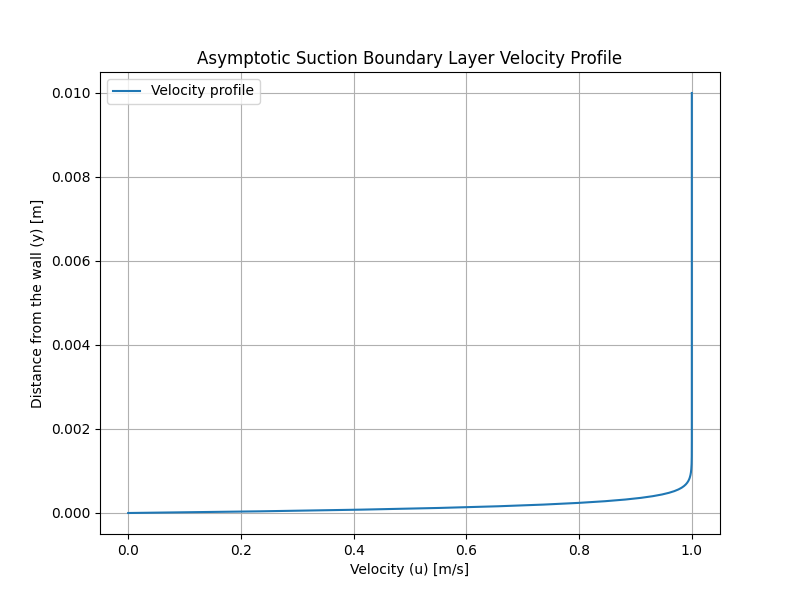
\includegraphics[width=0.4\textwidth]{output_plot.png}
    \caption{Numerical solution of suction boundary layer scenario showing the velocity profile.}
    \label{fig:suction boundary layer_solution}
\end{figure}

In addition, we have implemented in our script the calculation of the friction coefficient and wall shear stresses, which result in:
\begin{itemize}
    \item \textbf{Wall Shear Stress (\(\tau_{\text{wall}}\)):} \(0.122500 \, \mathrm{N/m^2}\)
    \item \textbf{Friction Coefficient (\(c_f\)):} \(0.2\)
\end{itemize}


\subsection{Calculation of the boundary layer displacement thickness}
The boundary layer displacement thickness (\(\delta^*\)) can be calculated by exploiting the definition of the velocity distribution into the formula provided by the excercise.
We start with the integral:

\[
\delta^* = \int_0^\infty e^{-\frac{V_w}{\nu} y} \, dy
\]
The integral of the exponential function is:
\[
\int e^{-\frac{V_w}{\nu} y} \, dy = -\frac{\nu}{V_w} e^{-\frac{V_w}{\nu} y} + C
\]

Now, we evaluate the definite integral from \(0\) to \(\infty\) and we get:
\[
u(y) = U_\infty \left(1 - e^{-\frac{V_w}{\nu} y}\right) = \frac{\nu}{V_w} = 0.000150 m
\]

\subsection{Applications of the suction boundary layer}
The suction boundary layer scenario finds applications in various engineering problems where boundary layer theory is relevant. One notable example is the flow over a long train, where the flow is parallel to the length of the train and the length is significantly greater than the width. 

\begin{thebibliography}{9}

\bibitem{NumericalMethods}
  \textit{Numerical and analytical solutions of new Blasius equation for turbulent flow},
  Mizanur Rahman, Shahansha Khan, M Ali Akbar.
\end{thebibliography}
\end{document}
